\usetikzlibrary{calc}
\begin{frame}{position independence cost (32-bit)}
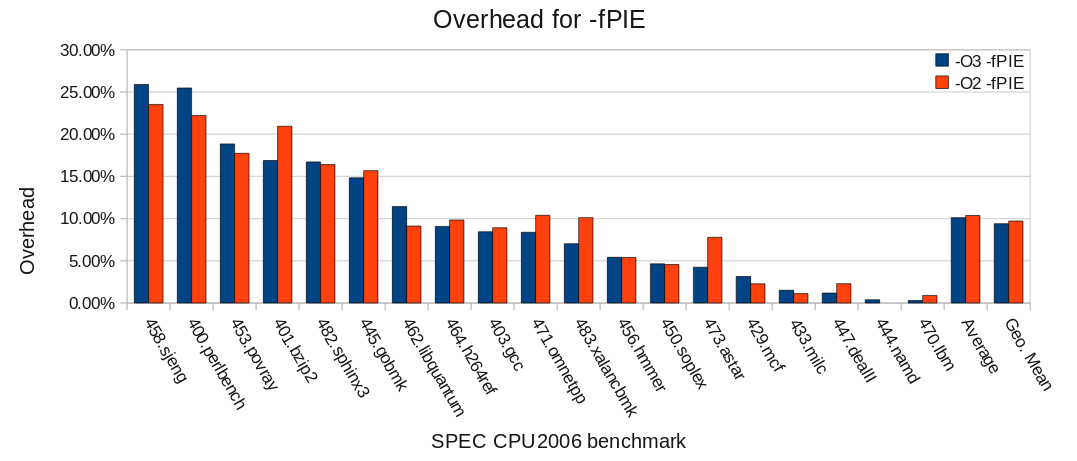
\includegraphics[width=\textwidth]{../mitigate/pie-cost}
\imagecredit{Payer, ``Too much PIE is bad for performance'', ETH Zurich Tech Report}
\end{frame}

\begin{frame}{position independence cost: Linux}
\begin{itemize}
    \item geometric mean of SPECcpu2006 benchmarks on x86 Linux
        \begin{itemize}
            \item with particular version of GCC, etc., etc.
        \end{itemize}
    \item 64-bit: 2-3\% (???)
        \begin{itemize}
        \item ``preliminary result''; couldn't find reliable published data
        \end{itemize}
    \item 32-bit: 9-10\%
    \item depends on compiler, \ldots
\end{itemize}
\end{frame}

\begin{frame}{position independence: deployment}
\begin{itemize}
    \item common for a very long time in dynamic libraries
    \item default for all executables in\ldots
    \vspace{.5cm}
    \item Microsoft Visual Studio 2010 and later
        \begin{itemize}
        \item \texttt{DYNAMICBASE} linker option
        \end{itemize}
    \item OS since 10.7 (2011)
    \item Fedora 23 (2015) and Red Hat Enterprise Linux 8 (2019) and later
        \begin{itemize}
        \item default for ``sensitive'' programs earlier
        \end{itemize}
    \item Ubuntu 16.10 (2016) and later (for 64-bit), 17.10 (2017) and later (for 32-bit)
        \begin{itemize}
        \item default for ``sensitive'' programs earlier
        \end{itemize}
\end{itemize}
\end{frame}

